\chapter{PRESENTATION OF PROJECT}

\section{General Presentation of Project}

\hs Machine learning and predictive models are widely used in various applications involving automated decision-making processes, such as classification, anomaly detection, forecasting, recommendation systems, and industrial data analysis. The performance of supervised learning models depends not only on the selected algorithms but also on the quality, completeness, and structure of the available data. The well-known principle of ``garbage in, garbage out'' (GIGO) highlights that incomplete, noisy, or poorly structured data can significantly reduce the accuracy and robustness of predictive systems.

In many real-world applications, datasets are often characterized by heterogeneous structures and multiple underlying distributions. In such cases, fitting a single global predictive model may be insufficient because the model may fail to capture local patterns or latent group-specific behaviors within the data. To address this issue, ensemble learning and aggregation techniques have been introduced to combine multiple predictive models and improve overall predictive performance.

This internship project focuses on the modular design and implementation of aggregation-based machine learning frameworks. The main objective is to study how multiple predictive models can be effectively combined using structured learning strategies, including \textbf{clusterwise modeling} and \textbf{kernel-based consensus aggregation}.

The proposed system is designed as a modular framework in which prediction is performed through a sequence of processing stages. It consists of two main components:

\begin{itemize}        
    \item \textbf{KFCProcedure}, which organizes the clusterwise learning workflow into three main steps:
          \begin{enumerate}        
              \item \textbf{K-Step:} detection of latent cluster structures in the dataset using clustering methods.
              \item \textbf{F-Step:} training of cluster-specific predictive models within the identified clusters.
              \item \textbf{C-Step:} combination of the predictions produced by the cluster-specific models.
          \end{enumerate}
          
          
    \item \textbf{GradientCOBRA}, which is a kernel-based aggregation method based on a distance-weighted consensus strategy. It combines multiple model outputs by measuring similarity in the prediction space and supports both internally trained and externally fitted predictive models.
          
\end{itemize}

Overall, the project aims to provide a unified and extensible framework for studying, implementing, and evaluating clusterwise learning and aggregation-based predictive modeling methods. The framework is designed to support consistent benchmarking, reusable software components, and seamless integration of diverse aggregation strategies.

\section{Problem Statement}

\hs The implementation and experimentation of aggregation methods and clusterwise predictive modeling techniques are often constrained by manual implementation and the lack of reusable, modular, and extensible software frameworks. This project addresses the following key problems:

\begin{itemize}        
    \item \textbf{Lack of Unified Architecture for Aggregation Methods:}
          Existing aggregation methods often share similar computational principles, such as prediction aggregation, distance computation, kernel weighting, optimization, and consensus strategies. However, they are commonly implemented as separate systems. The absence of a unified architecture makes it difficult to compare, extend, and integrate multiple aggregation techniques within the same framework.
          
          
    \item \textbf{Limited Modularity and Extensibility:} 
          Existing implementations of aggregation-based methods may not provide sufficient modularity and flexibility for deeper experimentation. When core components are tightly coupled, researchers may face difficulties in replacing base estimators, distance functions, normalization techniques, optimization procedures, or kernel functions. As a result, extending the framework to support new aggregation approaches or externally trained predictive models can require significant modification of the original implementation.
          
    \item \textbf{Complexity of Kernel-Based Consensus Aggregation:} 
          Kernel-based aggregation methods involve several interrelated processing stages, including data splitting, estimator training, prediction normalization, distance computation, kernel weighting, bandwidth optimization, loss evaluation, and final aggregation. Without a well-organized modular pipeline, managing these stages within a reusable and maintainable software structure becomes complex.
          
    \item \textbf{Difficulty in Handling Heterogeneous Data Distributions:} 
          A single traditional predictive model may be unable to adequately represent the latent structures, local patterns, or heterogeneous distributions commonly present in real-world datasets. Clusterwise learning techniques, such as the KFCProcedure, address this limitation by combining clustering, local model fitting, and prediction aggregation. However, implementing such workflows within a reusable and extensible framework remains challenging. This motivates the use of KFCProcedure, which is particularly suitable for situations where the input feature space contains unknown latent clusters and where the underlying predictive model may differ from one cluster to another.
          
\end{itemize}

To address these problems, this project focuses on packaging GradientCOBRA and KFCProcedure using a unified architecture that supports flexible experimentation, reusable components, maintainable implementation, and future extension.

\section{Objectives}

\hs The primary objective of this project is to design and develop modular Python libraries for clusterwise predictive modeling and kernel-based aggregation methods based on existing research literature.

The project specifically aims to achieve the following objectives:

\begin{itemize}        
    \item \textbf{Study} and understand the theoretical concepts related to Combined Classifier, MixCOBRA, GradientCOBRA, and KFCProcedure.
    \item \textbf{Redesign} existing implementations into a unified architecture with reusable pipeline components for data splitting, base estimators, normalization, distance functions, kernel functions, optimization procedures, and aggregation strategies.
    \item \textbf{Implement} the GradientCOBRA and KFCProcedure frameworks while improving extensibility, maintainability, and reusability.
    \item \textbf{Evaluate} the models from each library on regression and classification tasks using simulated and real-world datasets.
    \item \textbf{Provide} practical examples, clear documentation, and a well-structured API design suitable for researchers and practitioners.
\end{itemize}

\section{Contribution to Sustainable Development Goals}

\hs This internship project is aligned with the United Nations Sustainable Development Goals (SDGs), particularly in the areas of innovation, education, and research collaboration \cite{un2015sdgs}. Although the project is technical in nature, its contribution is not limited to algorithm implementation. By developing reusable machine learning libraries, the project supports the creation of digital research infrastructure that can be used for experimentation, learning, and future applied studies. The SDGs most closely related to this project are shown in Figure~\ref{fig:sdg_alignment}.

The main SDG related to this project is \textbf{SDG 9: Industry, Innovation and Infrastructure}. The \KFCProcedure{} and \GradientCOBRA{} libraries contribute to this goal by transforming advanced machine learning methods into modular, extensible, and reusable Python frameworks. This supports innovation in data science research by making clusterwise predictive modeling and aggregation-based learning easier to implement, compare, and extend.

The project also supports \textbf{SDG 4: Quality Education}. The developed libraries, examples, and documentation can help students, researchers, and practitioners understand advanced supervised learning methods through practical implementation. In this way, the project contributes to technical learning, research capacity building, and the development of data science skills.

In addition, the project indirectly supports \textbf{SDG 17: Partnerships for the Goals}. Since the work was conducted in an academic research laboratory and designed as reusable software, it encourages collaboration, reproducibility, and knowledge sharing among students, researchers, and future developers.

\begin{figure}[H]
\centering

\includegraphics[width=0.23\textwidth]{figures/sdg/9.png}\hfill

\includegraphics[width=0.23\textwidth]{figures/sdg/4.png}\hfill
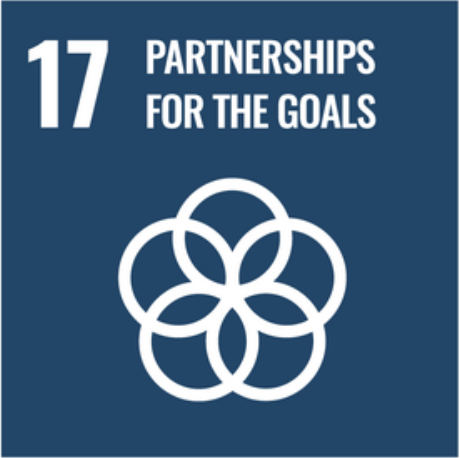
\includegraphics[width=0.23\textwidth]{figures/sdg/17.png}
\caption[SDGs contribution with the KFCProcedure project]{SDGs contribution with the KFCProcedure project: SDG 9, SDG 4, and SDG 17.}
\label{fig:sdg_alignment}
\end{figure}


\section{Planning of Project}

\hs To complete the project within the internship period, I followed a structured planning approach. The project was divided into four main phases, with each phase focusing on a specific part of the development process. This planning helped maintain a clear workflow, manage time effectively, and track progress throughout the internship. The overall project schedule is illustrated in Figure~\ref{fig:timeline}, which presents the timeline of activities across the different phases.

\begin{figure}[H]
    \centering
    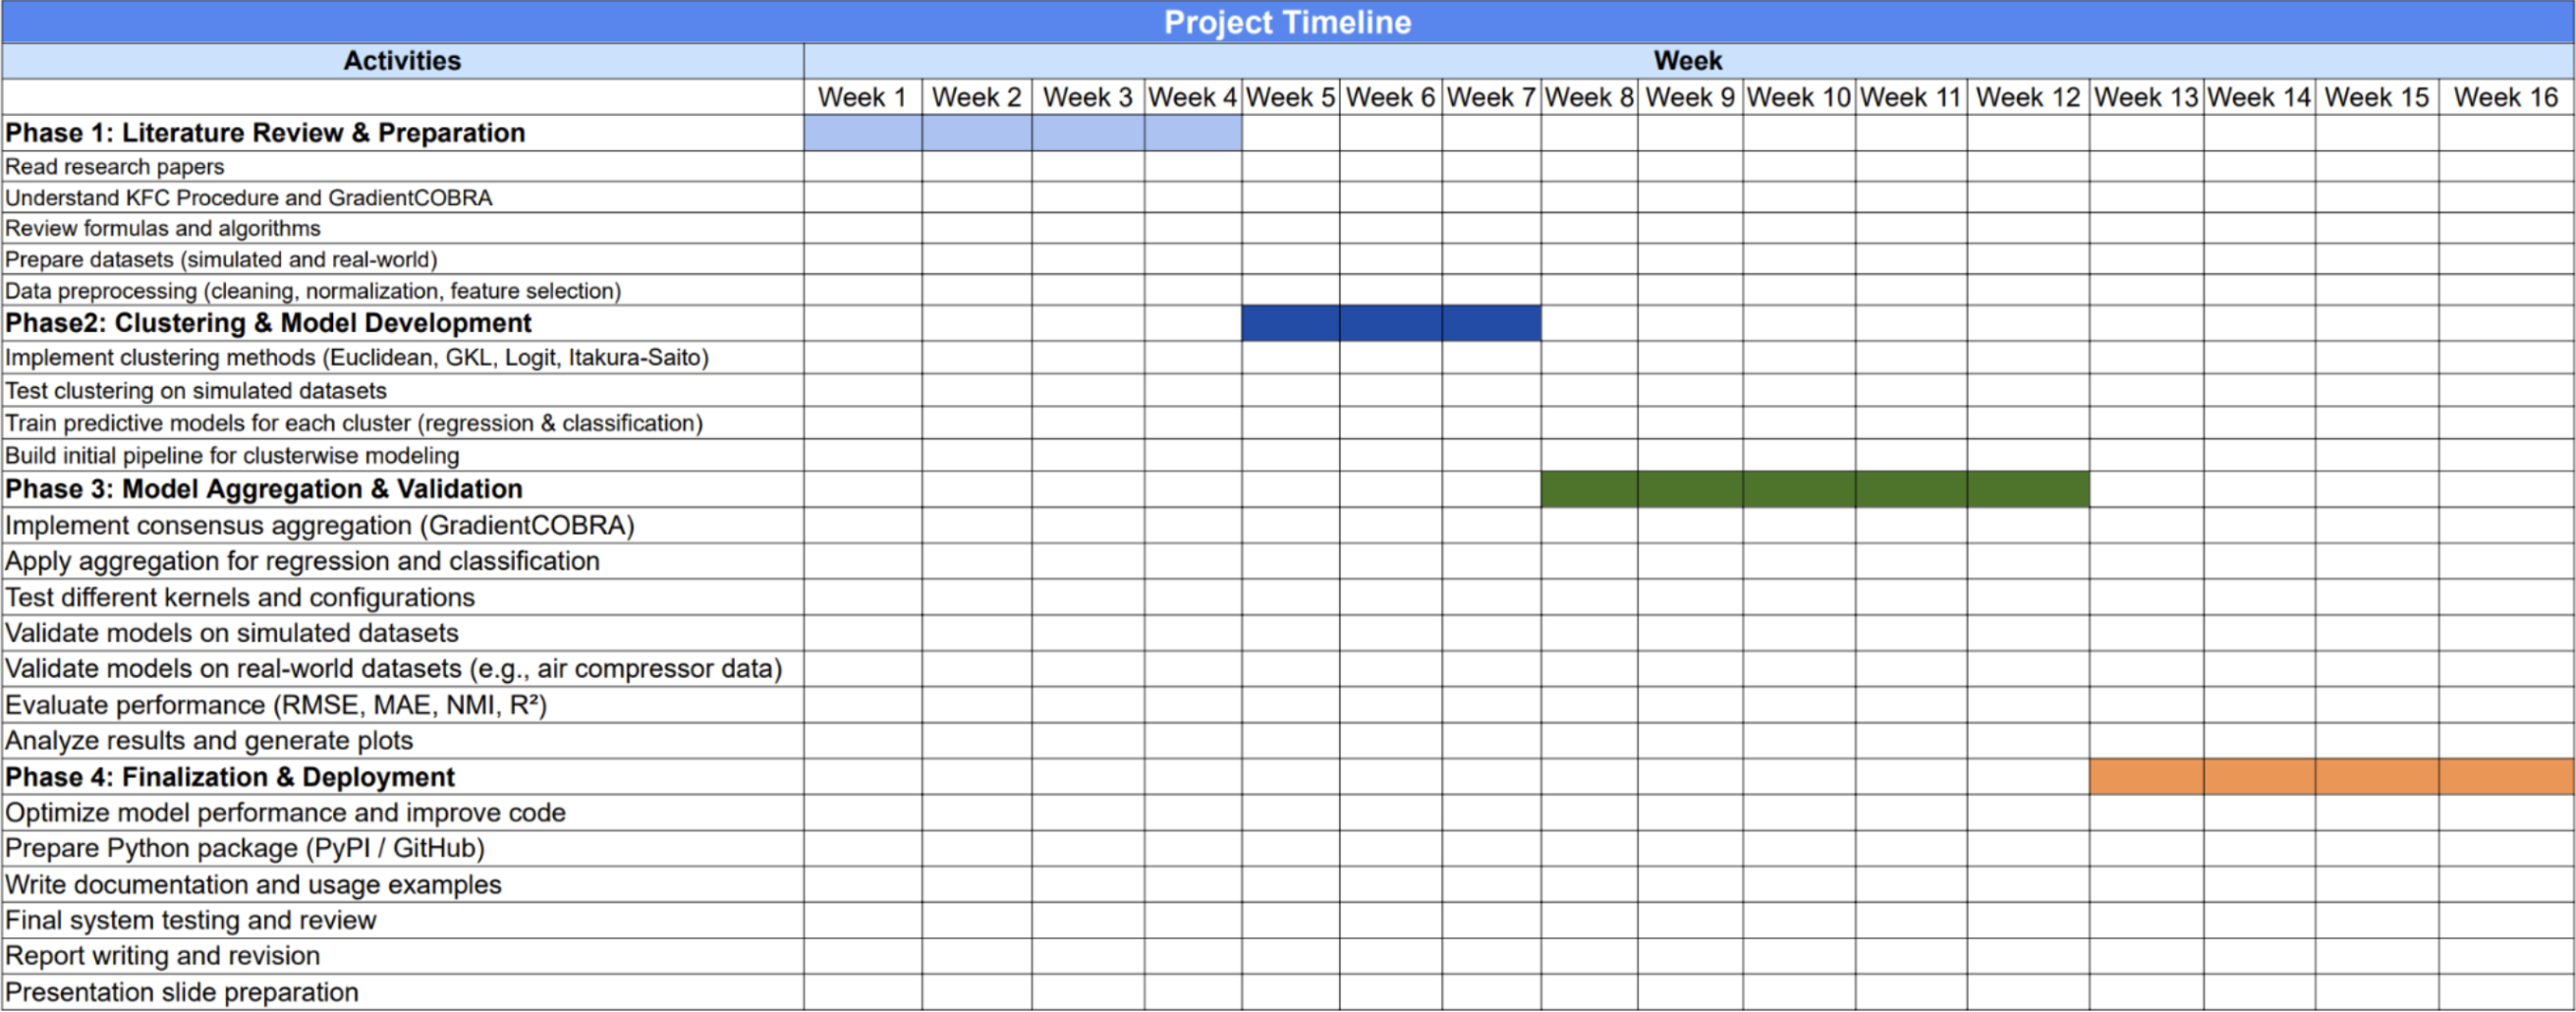
\includegraphics[width=1\textwidth]{figures/timeline.png}
    \caption{Project implementation timeline}
    \label{fig:timeline}
\end{figure}

